% It also requires running BibTeX. The commands are as follows:
%
%  1)  latex  aipsamp
%  2)  bibtex aipsamp
%  3)  latex  aipsamp
%  4)  latex  aipsamp
% Use the file aiptemplate.tex as a template for your document.
\documentclass[%
 aip,
%jmp,%
%bmf,%
%sd,%
rsi,%
 amsmath,amssymb,
%preprint,%
 reprint,%
%author-year,%
author-numerical,%
]{revtex4-1}
\usepackage{tabu}
\usepackage{graphicx}% Include figure files
\usepackage{dcolumn}% Align table columns on decimal point
\usepackage{bm}% bold math
\usepackage{float}
%\usepackage[mathlines]{lineno}% Enable numbering of text and display math
%\linenumbers\relax % Commence numbering lines

\begin{document}

\preprint{AIP/123-QED}

\title[Physics 111B - Optical Pumping (OPT) Lab]{Optical Pumping of Rubidium Vapor}


\author{Brandon Tran}
 \email{brandontran@berkeley.edu.}
\author{Lab Partner: Lok Ching Lui}%
\affiliation{$^1$Department of Physics, University of California, Berkeley%\\This line break forced with \textbackslash\textbackslash
}%


\date{\today}

\begin{abstract}

In this experiment, $^{85}Rb$ and $^{87}Rb$ atoms were optically pumped to higher energy levels. Incorporating the Zeeman effect using a modulating magnetic field and a radiofrequency (RF) field, these atoms were continuously pumped and "de-pumped." Measurements of the resonance frequency and magnetic field values allowed a calculation of the Zeeman energy levels of these atoms. Using the Breit-Rabi equation, the nuclear spins of $^{87}Rb$ and $^{85}Rb$ were determined to be $1.520\pm0.017$ and $2.542\pm0.032$, respectively. The magnitude of Earth's magnetic field at the location of Berkeley's Physics 111 Laboratory was also calculated to be 0.314 $\text{Gauss}\pm0.029$ Gauss from the data.

\end{abstract} 

\keywords{rubidium gas, optical pumping, Zeeman levels, nuclear spin, field modulation}

\maketitle


\section{Introduction} \label{1}
Optical pumping is a process in which light is used to raise or "pump" electrons in an atom from a lower energy level to a higher one. In this specific experiment, circularly polarized light was used in conjunction with the Zeeman effect (in a weak magnetic field), to move electrons in $^{85}Rb$ and $^{87}Rb$ atoms to their highest ground state Zeeman sublevel. \newline
\indent The technique of optical pumping was developed by Nobel Prize winner Alfred Kastler and is often used in the construction of lasers. where population inversion is achieved by pumping the active laser medium. Along with laser construction, optical pumping has many wide spread applications that include precise measurements of hyperfine level splittings in atoms and atomic clocks, measurements of weak magnetic fields, and MRI enhancement.\cite{Arditi} \newline
\indent In this paper, calculations of the nuclear spins of $^{85}Rb$ and $^{87}Rb$ and the Earth's magnetic field will be obtained by a measurement of the resonant frequency and magnetic field values that match the Zeeman energy level splittings of the rubidium atoms. Section \ref{2} describes the relevant atomic theory to understand optical pumping and how optical pumping works, section \ref{3} and \ref{4} describes the setup and procedure in this experiment, and section \ref{5} describes the results of our experiment.

\section{Background \& Theory} \label{2}
This section describes the energy structure of the rubidium atom. Along with a discussion of the Zeeman effect, a detailed explanation of how optical pumping works will be discussed. We assume the reader is familiar with the finer details of the atomic energy splittings associated with the fine and hyperfine levels.

\subsection{Atomic Structure and Energy Levels}
Electrons in atoms are bounded by potentials that give rise to quantized energy levels. Referring to Fig.~\ref{fig:Rb85structure} and Fig.~\ref{fig:Rb87structure}, the principal energy state or hydrogenic state arises from the coulomb interaction between the positively charged nucleus and the negatively-charged electrons. \newline
\indent However, due to relativistic corrections and the spin-orbit coupling of electrons, these hydrogenic states split further, giving rise to the fine structure or electron spin-orbit structure. Because the electron has spin, the total angular momentum of the electron can be described by its orbital angular momentum l and its spin number s. In vector notation, the total angular momentum $\bf{J}$ of the electron is 

\begin{equation}
\bf{J}=\bf{L}+\bf{S}
\label{eq:one}
\end{equation}

\noindent where $\bf{S}$ is the spin of the electron and $\bf{L}$ is the orbital angular momentum of the electron. The fine structure splits the gross structure into states with  $L-S\leq J \leq L+S$.

\indent A further splitting arises due to the interaction between the nuclear magnetic dipole moment and the magnetic moment of the electrons. This splitting causes the hyperfine structure or the electron/nuclear spin structure. Because the nucleus has a spin $\bf{I}$ associated with it, the total angular momentum of the atom $\bf{F}$ is then defined as

\begin{equation}
\bf{F}=\bf{J}+\bf{I}
\label{eq:two}
\end{equation}

\noindent The hyperfine structure splits the fine structure into states with  $I-J\leq F \leq I+J$.


The rubidium atom, whose electron configuration is 

\begin{equation}
1 s ^ { 2 } 2 s ^ { 2 } 2 p ^ { 6 } 3 s ^ { 2 } 3 p ^ { 6 } 3 d ^ { 10 } 4 s ^ { 2 } 4 p ^ { 6 } 5 s
\label{eq:three}
\end{equation}

\noindent has only one valence electron in the 5s state. Because all of the other electrons are tightly bounded, this experiment will focus on this lone "optically active" valence electron.

Referring to Fig.~\ref{fig:Rb85structure} and Fig.~\ref{fig:Rb87structure} for the rubidium atom, another splitting occurs to the hyperfine levels when atoms are present in a weak external magnetic field, $\bf{B}_{ext}$. This is called the Zeeman effect and gives rise to the Zeeman splittings.

\begin{figure}[H]
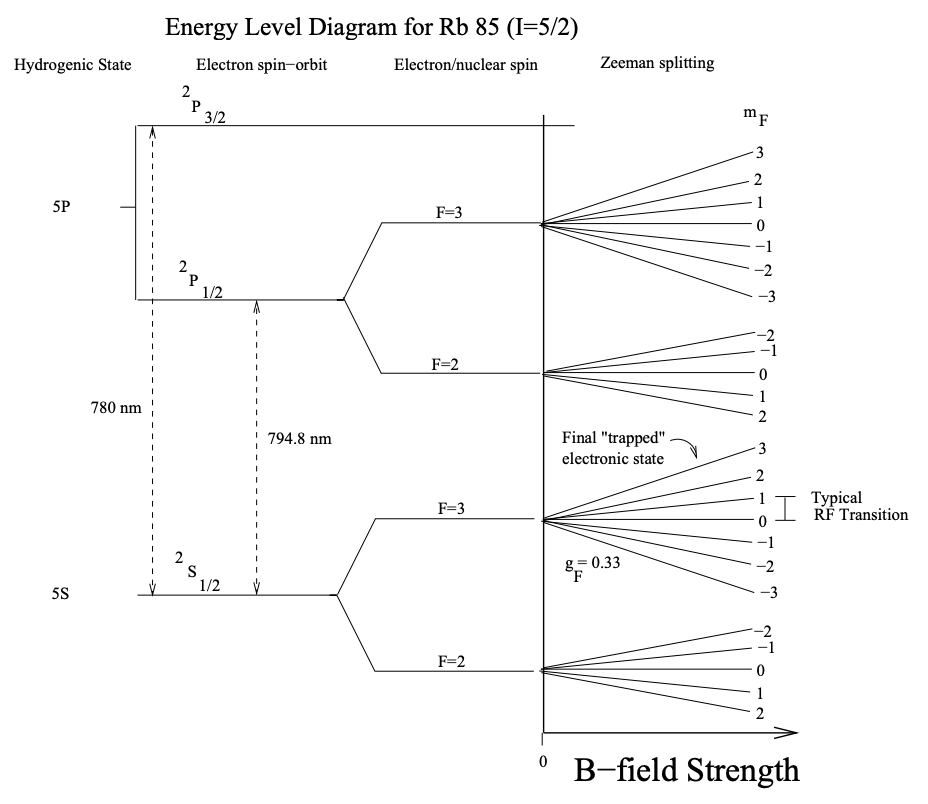
\includegraphics[width=1\linewidth]{lateximages/Rb85structure.png} 
\caption{\label{fig:Rb85structure}  Energy levels and splittings in $^{85}Rb$. }
\end{figure}

\begin{figure}[H]
\center
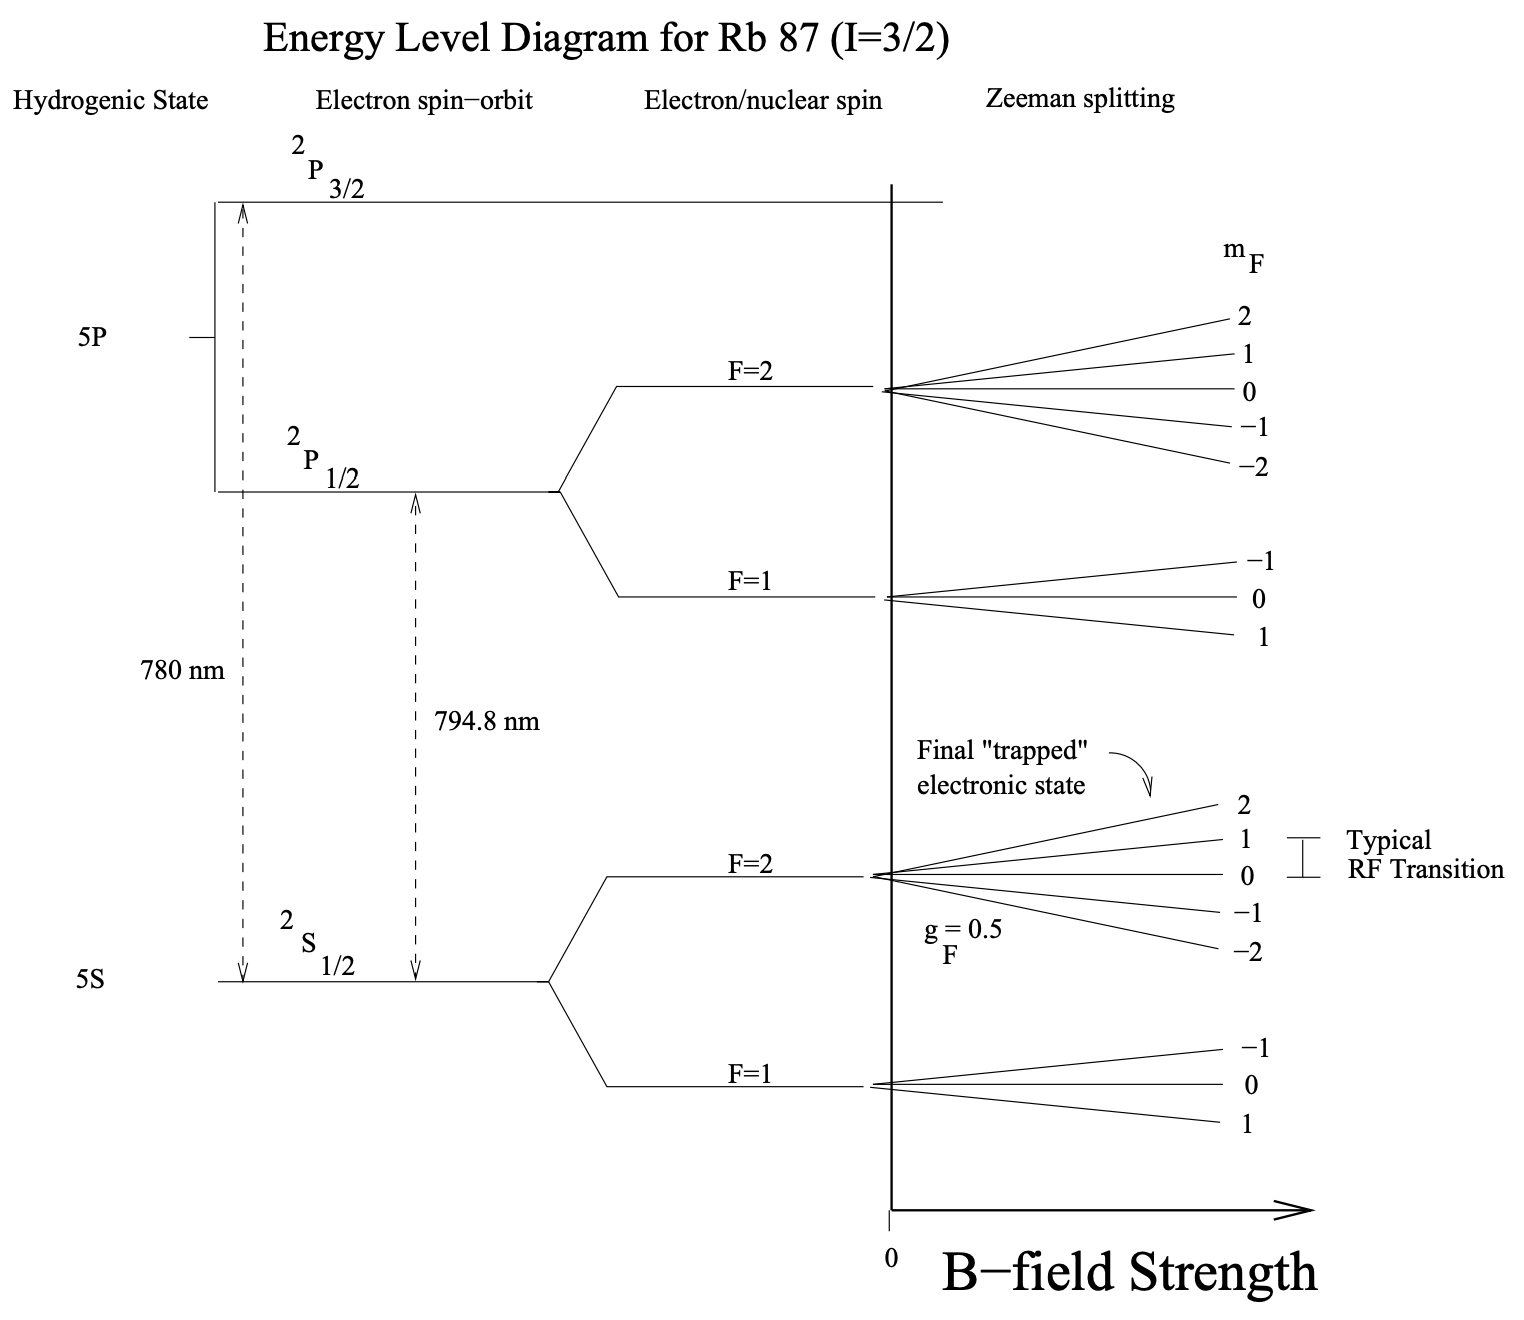
\includegraphics[width=1\linewidth]{lateximages/Rb87structure.png}
\caption{\label{fig:Rb87structure}  Energy levels and splittings in $^{87}Rb$. }
\end{figure}

For a given F, the Zeeman effect causes the hyperfine levels to split into 2F+1 levels with the $m_{F}$ values ranging from $-F\leq m_{F} \leq F$. The energy of these Zeeman levels is given by 

\begin{equation}
E = E _ { 0 } + g _ { f } m _ { f } \mu _ { B } B_{ext}
\label{eq:four}
\end{equation}


\noindent where $E _ { 0 }$ is the energy of the eigenstate when $\bf{B}_{ext}$ is zero, $\mu _ { B }$ is the Bohr magneton, and $g _ { f }$ is the Land\'e g-factor, defined as 

\begin{equation}
g _ { F } = g _ { J } \frac { F ( F + 1 ) + J ( J + 1 ) - I ( I + 1 ) } { 2 F ( F + 1 ) }
\label{eq:five}
\end{equation}

\noindent and 

\begin{equation}
g _ { J } = 1 + \frac { J ( J + 1 ) + S ( S + 1 ) - L ( L + 1 ) } { 2 J ( J + 1 ) }
\label{eq:six}
\end{equation}

The energy difference between adjacent Zeeman levels for a given F is then given by 

\begin{equation}
\Delta E _ { \mathrm { Zeeman } } = g _ { F } \mu _ { B } B_{ext}
\label{eq:seven}
\end{equation}

Now, in this experiment, we will only focus on the Zeeman splittings in the highest F ground state of rubidium. For the ground state of rubidium s=$\frac{1}{2}$ and l=0, so j=$\frac{1}{2}$. Noting that $\Delta E _ { \mathrm { Zeeman } }$ is just $h\nu$ and F=I+J, Eq.~\ref{eq:seven} can be rewritten as 

\begin{equation}
\frac { \nu } { B _ { \mathrm { ext } } } = \frac { 2.799 } { 2 I + 1 } \mathrm { MHz } / \mathrm { gauss }
\label{eq:eight}
\end{equation}

\noindent which is known as the Breit-Rabi equation. 


\subsection{Optical Pumping}
Consider Fig.~\ref{fig:Rb87structure} of the $^{87}Rb$ structure and the effect of shining left-circularly polarized light on $^{87}Rb$ vapour with Zeeman splitting in a weak magnetic field. Focusing on the ground state $^{2} S _ { 1 / 2 }$ and the first excited state $^{2} P _ { 1 / 2 }$ levels, when resonant optical light is incident on the rubidium vapour and is absorbed, the electron in the ground state $^{2} S _ { 1 / 2 }$ will make a transition into the $^{2} P _ { 1 / 2 }$ level. Since the light is circularly polarized (carrying one unit of angular momentum) and if we shine in the direction of the external magnetic field, however, then the absorption of the photon must mean that $\Delta m_{f}=+1$. So an electron in F=1 and $m_{f}=-1$ ground state can only transition to a substate with $m_{f}=0$ in the excited state.\cite{Zafra} \newline
\indent When this electron falls back down to its ground state due to spontaneous emission, however, dipole radiation rules allow for $\Delta m_{f}=0, \pm1$ with equal probability, meaning it has a $\frac{2}{3}$ chance of having a higher $m_{f}$ value than it was before when it was in the ground state. The atom will absorb and reradiate again, and if nothing happens to disturb the Zeeman levels during this process, all the atoms will be "pumped" into the F=2 and  $m_{f}=2$ state after multiple absorptions and emissions. Moreover, when the atom reaches this level, it can no longer absorb the resonant photons because there does not exist a state with $m_{f}=3$ in this example and conservation of momentum dictates $\Delta m_{f}=+1$ upon absorption.  Referring to Fig.~\ref{fig:Rb85structure} and Fig.~\ref{fig:Rb87structure}, the final pumped states of  $^{85}Rb$ and $^{87}Rb$ are the F=3, $m_{f}=3$ and F=2, $m_{f}=2$ levels of the $^{2} S _ { 1 / 2 }$ state, respectively.  This technique of raising the energy levels of the atom is called optical pumping. \newline
\indent When pumping is achieved, the rubidium vapour becomes transparent to the polarized light as it can no longer absorb any more. By introducing a radiofrequency (RF) radiation with the energy equal to the Zeeman splitting energy, $\Delta E _ { \mathrm { Zeeman } }=h\nu$, where $\nu$ is the frequency of the light, the saturated pumped levels can be "depumped" into lower Zeeman levels to allow pumping to occur again.

\begin{figure}[H]
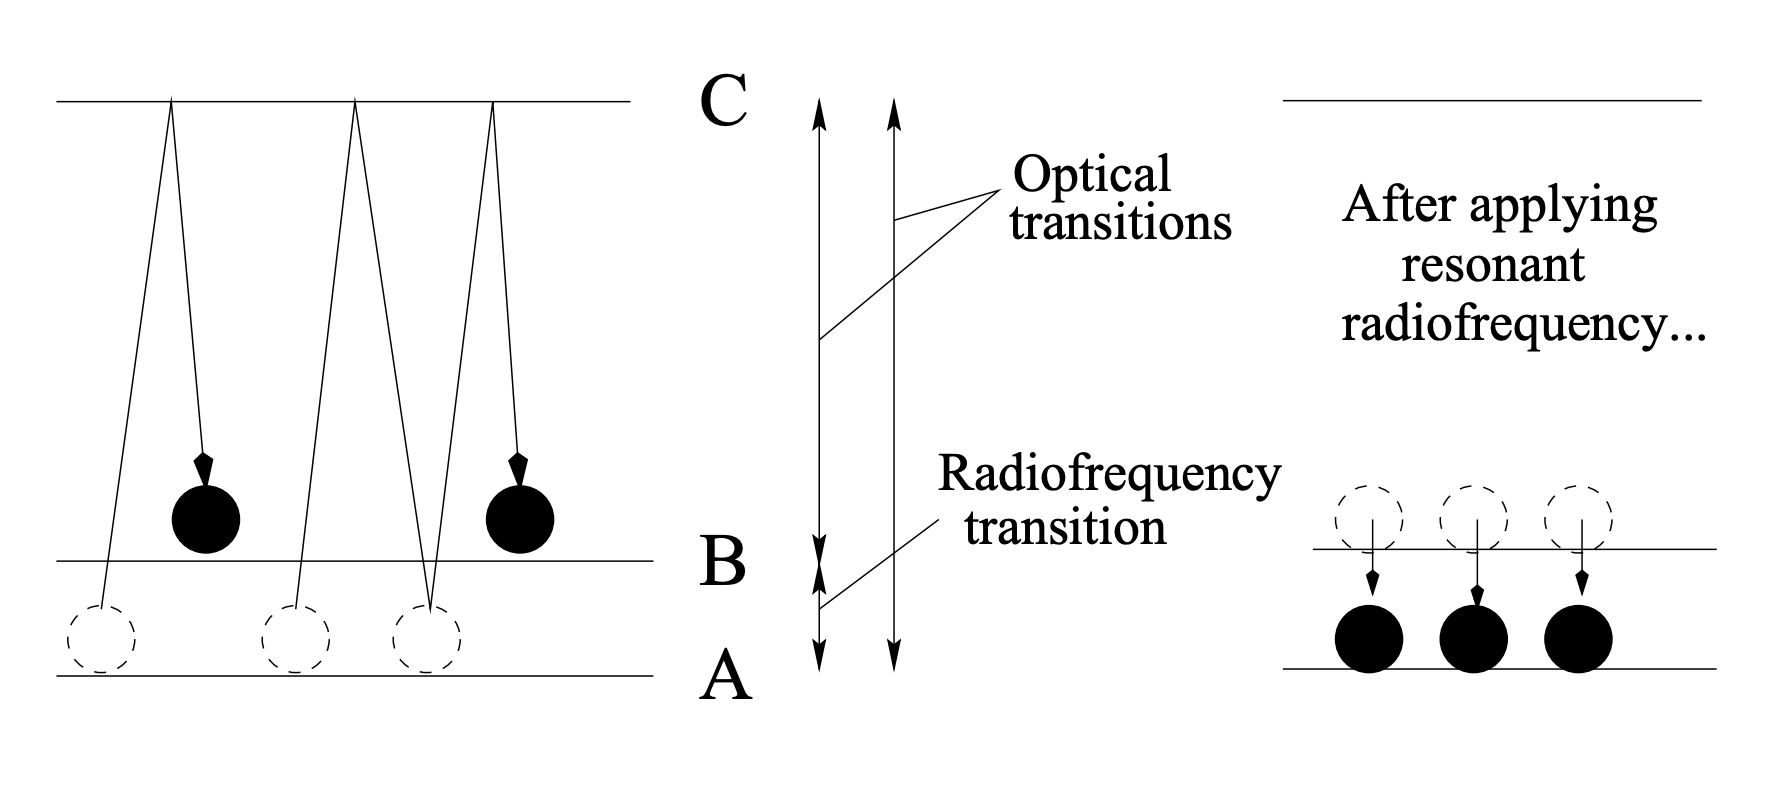
\includegraphics[width=1\linewidth]{lateximages/opticalpumping.png} 
\caption{\label{fig:opticalpumping}  Simple illustration of optical pumping. Adapted from [3]. }
\end{figure}

Fig.~\ref{fig:opticalpumping} illustrates this process of pumping and depumping. Atoms in the ground state A can be pumped into the state B through continuous iterations of absorbing and emitting optical radiation. When all the atoms end up in state B, pumping can no longer occur. But by applying a resonant RF field equal to the Zeeman splitting, transitions from B to A can be induced, and pumping can occur again. Looking back at Eq.~\ref{eq:eight}, the Breit-Rabi equation, one can see that the resonant RF frequency depends linearly on the strength of the externally applied magnetic field. By measuring the resonant frequencies at various externally applied magnetic fields or vice versa, one can determine the nuclear spins of the rubidium atoms.

\section{Experimental Setup} \label{3}
The experimental setup is shown on Fig.~\ref{fig:equipment} on the next page. The rubidium lamp provides the optical pumping light by traveling through a circular polarizer and a D1 filter. By applying this polarized light at the proper frequency using the D1 filter, transitions from the ground state to the excited states of the rubidium atoms can be induced. The light intensity from the rubidium lamp is detected by the photodiode. When all the atoms are pumped, we see an increase in light intensity detected as no more photons can be absorbed. By introducing a radiofrequency signal of the right frequency to stimulate transitions to lower Zeeman levels, a decrease in signal intensity will be detected in the photodiode as the system is being pumped again.

\begin{figure*}
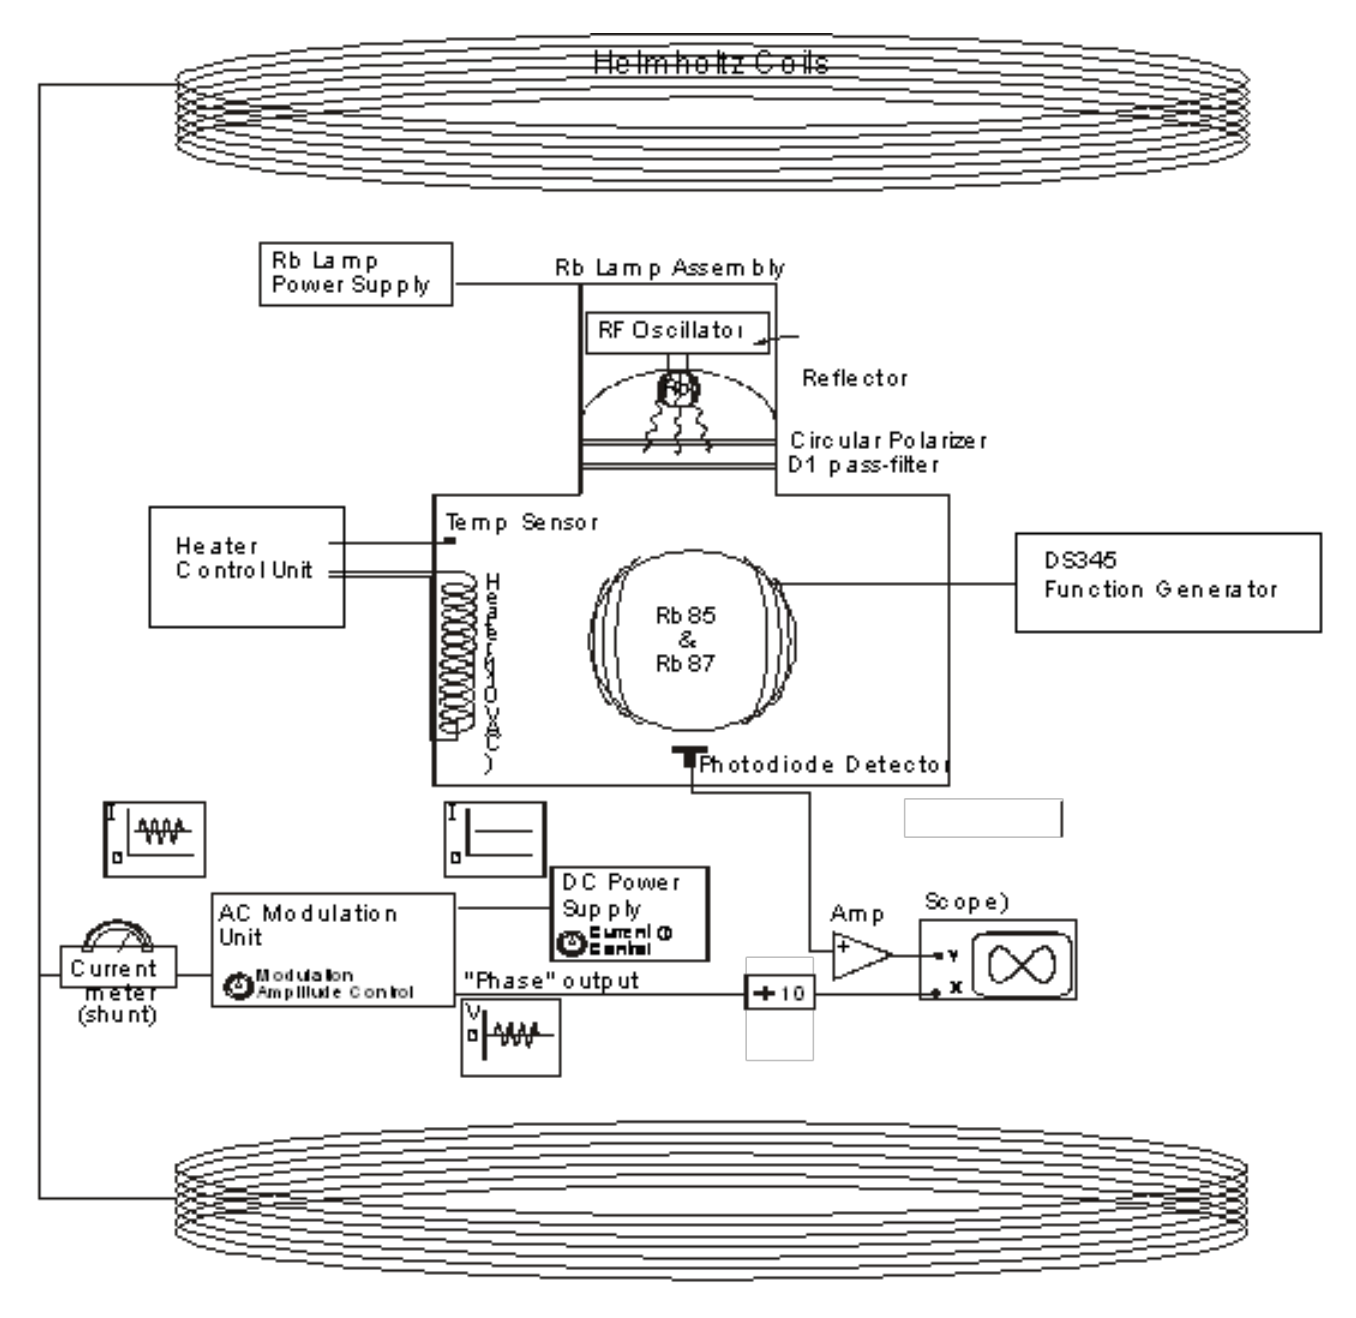
\includegraphics[width=0.9\linewidth]{lateximages/equipment} 
\caption{\label{fig:equipment}  Experimental setup for optical pumping. Adapted from [4]. }
\end{figure*}

\subsection{Helmholtz Coils}
The Helmholtz coils provide the weak magnetic field needed to provide Zeeman splitting to the atoms. It is powered by a DC power supply and can also be modulated using an AC modulation unit. The number of turns of the coils is N=135 and its radius is R=27.5 cm. The strength of this magnetic field, which determines the strength of the resonant RF frequency, can be determined by considering the magnetic field at a distance z from the center of a loop of current. Recall the formula is 


\begin{equation}
\mathbf { B }_{H} ( z ) = \frac { \mu _ { 0 } i } { 2 } \frac { R ^ { 2 } } { \left( R ^ { 2 } + z ^ { 2 } \right) ^ { 3 / 2 } } \hat { \mathbf { z } }
\label{eq:nine}
\end{equation}

By placing two loops at a distance $\pm\frac{R}{2}$ and using superposition, the magnetic field at the rubidium sample becomes

\begin{equation}
\mathbf { B }_{H} ( 0 ) = \frac { 8 \mu _ { 0 } i } { 5 \sqrt { 5 } R } \hat { \mathbf { z } }
\label{eq:ten}
\end{equation}

Using $\mu_{0}=4\pi \times 10^{-7}$ and N coils, we then have the magnetic field of the Helmholtz coils is then

\begin{equation}
B _ { H } = 0.9 \times 10 ^ { - 6 } \cdot \frac { N i } { R } \,\, Tesla
\label{eq:eleven}
\end{equation}

\noindent Then we can determine the Helmholtz field by measuring the current i passing through it.

\subsection{Rubidium Bulb or Cell}
The rubidium bulb contains the $^{85}Rb$ and $^{87}Rb$ atoms and is vaporized using the heater control unit. The bulb contains a low density of rubidium atoms and is mixed with a buffer gas to minimize the mixing of states. To achieve pumping, the rubidium bulb must be heated by the control unit so that it remains in a vapor state. \newline 
\indent As in Fig.~\ref{fig:equipment}, the radiofrequency signal is provided by the coils surrounding the rubidium lamp and the function generator connected to it.  Without the RF field, the atoms will be all pumped eventually, and a maximum photodiode signal will be present. The RF provides a change in this photodiode signal by  depumping the atoms into lower Zeeman levels so that pumping can occur again.



\section{Procedure} \label{4}
Since the main goal of this experiment is to calculate the nuclear spins of the rubidium isotopes and Earth's magnetic field, a determination of the resonant RF frequency $\nu$ values and the associated external magnetic field $\bf{B}_{ext}$ needs to be carried out to use in the Breit-Rabi equation. The resonant RF frequency can be determined in one of two ways: modulating the RF frequency or modulating the magnetic field. 

\subsection{RF Frequency Modulation}
By sweeping through the values of the RF frequency for a given Helmholtz field, we can find the resonance frequency needed to induce stimulated emission in the rubidium vapor. \newline
\indent First, the sample is heated to a sufficient amount and a 1A DC current is driven through the Helmholtz coil to start with. This induces Zeeman splittings in the rubidium atoms and the strength of this current determines the strength of the resonant RF frequency between the Zeeman levels. The RF frequency is driven using a DS345 function generator with a carrier wave centered at around approximately 2.8MHz with a ramp frequency modulation. \newline
\indent The signal from the photodiode is sent into a preamp and then CH2 of the oscilloscope and the function generator output is sent to CH1. As the resonant RF field depumps electrons into lower $m_{f}$ levels, these depumped atoms can now be pumped, and the changes in opacity (indicated by a dip in the photodetector output) shows that the atoms are absorbing light and being pumped. \newline
\indent By changing the carrier RF frequency and the span, we can search for resonance on the oscilloscope by noting the opacity changes as a function of frequency. When resonance is found, a more accurate reading of the resonant frequency can be made by reducing the span of our modulated wave to "hone" in on the resonance. This process can be repeated by changing the DC current value powering the Helmholtz coils and finding the new resonance value by the method above. \newline
\indent Although this method works to find resonance, it is not as accurate as modulating the magnetic field. This is because RF frequency and the function generator can only be changed in discrete steps whereas the current driving the magnetic field can be changed continuously by a current knob.

\begin{figure}
\center
\includegraphics[width=1\linewidth]{lateximages/lissajous}
\caption{\label{fig:lissajous}  Oscilloscope traces of Lissajous curves. Adapted from [5]. }
\end{figure}

\subsection{Magnetic Field Modulation}
Instead of the RF frequency modulation, the magnetic field provided by the Helmholtz coil can be modulated. This provides a quicker and more accurate way of finding the resonance frequency. Turning off the RF frequency modulation and driving the function generator powering the RF coils at a fixed frequency, we can search for resonance by a magnetic field modulation. Referring to Fig.~\ref{fig:equipment}, the AC modulation unit was turned on and was modulated at a value big enough to show the changes in opacity. \newline
\indent The phase out signal of the AC modulation unit is now connected to CH1 of the scope instead of the function generator's output and the scope was set to XY mode. We should observe what is known as a Lissajou curve on the scope as can be seen in Fig.~\ref{fig:lissajous}. \newline
\indent By changing the current powering the Helmholtz coils, we can find resonance by noting that the Lissajous curve should be symmetric about the y-axis. This indicates that there is an equal change in transparency about the DC current value and thus this current matches the fixed resonance frequency of the splitting. \newline
\indent This Lissajous curve can be explained by a simple model in which the modulated magnetic field of the Helmholtz coils is of the form $B _ { H }=sin(t)$ and at resonance the photodetector output should be of the form $sin^2(t+\phi)$, where t is the time and $\phi$ is a phase shift that can be controlled on the coil driver panel. \newline
\indent By changing the value of the fixed RF frequency and searching for resonance by varying the current driving the modulating magnetic field, we can note at what magnetic field values gives the resonant frequency by noting the symmetry of the Lissajous curve. To obtain a more accurate measurement, the modulation amplitude can be adjusted even smaller to hone in on the resonance.


\section{Results and Analysis} \label{5}
This section contains the main results of this experiment. We first note how the signal intensity from the photodiode depends on the temperature of the rubidium isotopes. We then find a resonance signal at zero external magnetic field. Lastly, the nuclear spins of the rubidium isotopes and the Earth's magnetic field value will be determined.

\subsection{Signal Intensity vs Temperature}
For optical pumping to occur, the temperature of the rubidium atoms must be high enough to that it is in a vapor state, and it must also be low enough to not cause mixing of states. \newline
\indent Heating the rubidium atoms off the wall into the rubidium cell will cause a higher vapor density that attenuates the rubidium lamp more when it is not optically pumped. As a result, the detected signal (the difference in optical transmission in the cell in the presence and absence of pumping) will be larger. When the temperature is too high, however, and the vapor density increases even further, Rb-Rb collisions and other effects like mixing reduce the lifetime of the optically pumped state and so reduces the signal. \newline
\indent By locating the resonant frequency values of each isotope and examining the photodiode detector signal on the scope, we find that the maximum signal for $^{85}Rb$ occurs when the temperature is at $38^{\circ}C$ and  $41^{\circ}C$ for $^{87}Rb$. 

\begin{figure*}
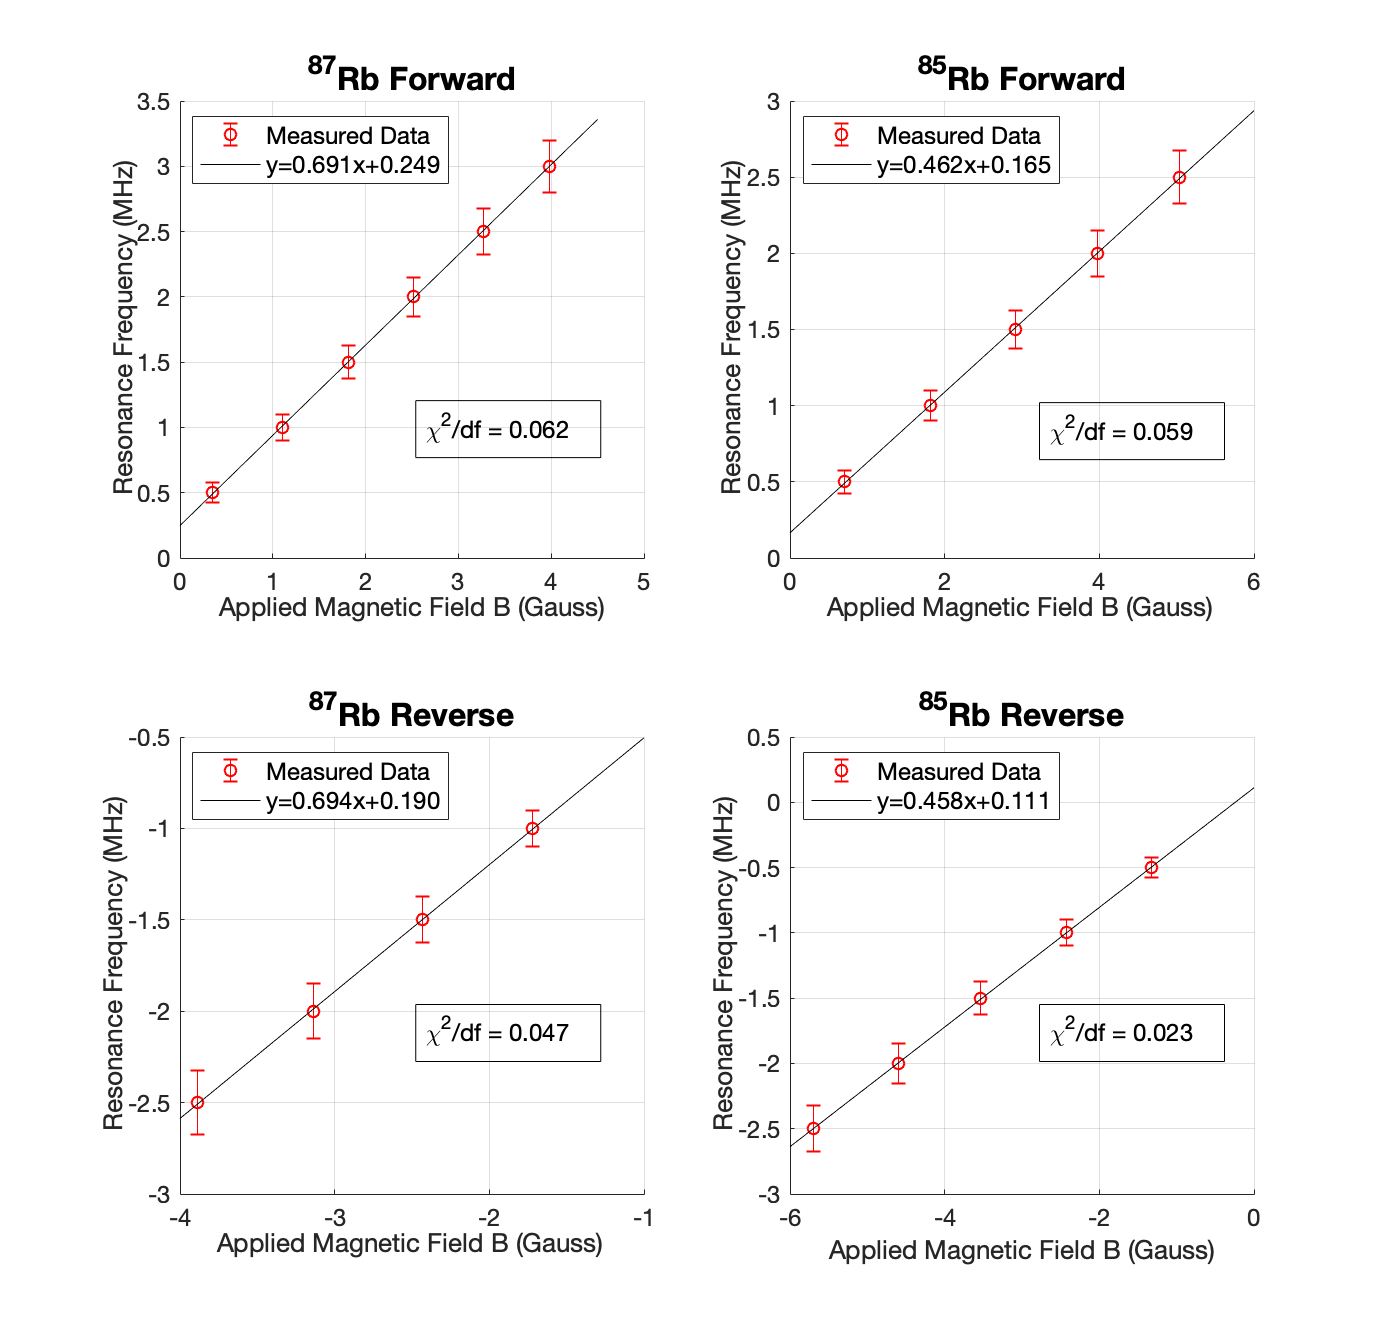
\includegraphics[width=1\linewidth]{lateximages/linear.png} 
\caption{\label{fig:linear}  Resonant RF frequencies as a function of the applied Helmholtz magnetic field $B_{H}$ for $^{85}Rb$ and $^{87}Rb$. }
\end{figure*}

\subsection{Zero Field Resonance}
With the RF field off and the magnetic field set in reverse polarity, we sweep the current driving the Helmholtz coils and find a resonance at a current of $0.1A\pm0.02A$. This corresponds to a magnetic field of about $0.442$ Gauss $\pm$ $0.088$ Gauss. This current should not exist if the Helmholtz coils were perfectly aligned with the Earth's magnetic field, and this nonzero current value of zero resonance indicates there are other external magnetic fields besides the Helmholtz coils. \newline
\indent Zero field resonance occurs when the applied Helmholtz field cancels the Earth's magnetic field, leading to an overall zero net external magnetic field. The Zeeman levels become degenerate, and there is no longer a distinction between the Zeeman levels. There can no longer be pumping of the atoms and a distinct dip in the scope indicates more light is being absorbed by the vapor.

\begin{table*}
\caption{\label{tab:table1}Nuclear Spin of $^{85}Rb$ and $^{87}Rb$  }
\begin{ruledtabular}
\begin{tabular}{ccccc}
\bf{Isotope} & \bf{Polarity} & \bf{Slope (MHz/Gauss)} & $\bf{I}_{calculated}$ & $\bf{I}_{actual}$\\ 
\hline
$^{85}Rb$ & Forward & $0.462\pm0.009$ & $2.530\pm0.054$ & $2.5$ \\
\hline 
$^{85}Rb$ & Reverse & $0.458\pm0.006$ & $2.555\pm0.036$ & $2.5$ \\
\hline
$^{87}Rb$ & Forward & $0.691\pm0.009$ & $1.525\pm0.022$ & $1.5$ \\
\hline
$^{87}Rb$ & Reverse& $0.694\pm0.012$ & $1.516\pm0.026$ & $1.5$ \\
\end{tabular}
\end{ruledtabular}
\end{table*}

\subsection{Determining the Nuclear Spins of $^{85}Rb$ and $^{87}Rb$ }
By finding the resonant RF frequency and magnetic field values from the Helmholtz coils by using the procedure described in the magnetic field modulation subsection, the Breit-Rabi equation (Eq.~\ref{eq:eight}) can then be used to find the nuclear spins of the rubidium isotopes. Fig.~\ref{fig:linear} shows the plots of resonant RF frequencies as a function of the Helmholtz field $B_{H}$ for both $^{85}Rb$ and $^{87}Rb$ in forward and reverse magnetic field polarities (and allowing "negative" frequencies). \newline
\indent A least-squares fit was performed for each set of data with associated chi-squared values displayed in the figure. Errors tended to increase as the magnitude of the magnetic current increased. These errors were calculated by noting the range of magnetic field values that seem to produce resonance as seen by the symmetry of the Lissajou curve on the scope and propagated to the frequency errors by using the Breit-Rabi equation. Multiple measurements of the resonant frequency values and errors were also made at each magnetic field value for a better error calculation. \newline
\indent From the least-squares fit, the slope can be calculated and therefore the nuclear spins of the isotopes can be determined. The results of these calculations using the data from Fig.~\ref{fig:linear} can be seen in Table~\ref{tab:table1}. \newline 
\indent From the slope calculations, the nuclear spins can be determined by noting from the Breit-Rabi equation that 

\begin{equation}
slope=\frac{2.799}{2I+1}
\label{eq:twelve}
\end{equation}

Calculating this for each of the four graphs and averaging the forward and reverse polarity values of each isotope in Table~\ref{tab:table1}, we determine that the nuclear spins of $^{85}Rb$ and $^{87}Rb$ are $I_{85}=2.542\pm0.032$ and $I_{87}=1.520\pm0.017$, respectively. Compared to the actual values of 2.5 and 1.5, these calculated values are within $2\%$ of the actual values.




\subsection{Calculation of Earth's Magnetic Field}
To determine the magnitude of Earth's magnetic field, we combine the data from the forward and reverse polarity of each isotope into two graphs, one for $^{85}Rb$ and one for $^{87}Rb$. These two new graphs are again fitted using the least-squares method. \newline
\indent Now there are two ways to calculate Earth's magnetic field, one is to see where the line crosses the x-axis and that is Earth's magnetic field value. The other way is to determine the y-intercept and noting that from the Breit-Rabi equation,

\begin{equation}
B _ { e x t } = B _ { H }+B_{Earth}
\label{eq:thirteen}
\end{equation}

\noindent Now the y-intercept is equal to 

\begin{equation}
y-intercept=\frac{2.799}{2I+1} \times B_{earth}
\label{eq:fourteen}
\end{equation}
\newline
The results of these calculations can be seen in Table~\ref{tab:table2}. By calculating the y-intercept for each of the isotopes and taking an average, we find that the magnitude of Earth's magnetic field is $B_{Earth}=0.314$ Gauss $\pm$ 0.029 Gauss.


\begin{table}[H]
\caption{\label{tab:table2}Earth's Magnetic Field  $B_{Earth}$ }
\begin{ruledtabular}
\begin{tabular}{ccccc}
\bf{Isotope} & \bf{y-intercept(MHz)} & $\bf{B}_{Earth}$ $\bf{(Gauss)}$\\ 
\hline
$^{85}Rb$  & $0.146\pm0.005$ & $0.314\pm0.010$ \\
\hline
$^{87}Rb$ &  $0.219\pm0.005$ & $0.314\pm0.07$  \\
\end{tabular}
\end{ruledtabular}
\end{table}

\section{Conclusion}
Through the optical pumping of rubidium vapor, the nuclear spins of $^{85}Rb$ and one for $^{87}Rb$ were calculated to be $2.542\pm0.032$ and $1.520\pm0.017$, respectively. These values are extremely accurate for an undergraduate laboratory. Earth's magnetic field was also determined to have a value of 0.314 Gauss $\pm$ 0.029 Gauss. The precision and ease of this experiment provides many practical applications from atomic clocks to MRI, and has provided great context for illustrating quantum mechanical concepts.


\begin{acknowledgments}
We would like to thank the Physics 111B staff for their patience and guidance during this experiment. Without you, we would still be trying to figure out how to setup the experiment. \newline

\end{acknowledgments}

   
\nocite{*}

 \begin{thebibliography}{1}
 
\bibitem{Arditi} M. Arditi, J.L. Picque, {\em "A cesium beam atomic clock using laser optical pumping,”} Journal de Physique Lettres (1980). \newline

\bibitem{Zafra} R.L. De Zafra, {\em "Optical Pumping,”} American Journal of Physics, 28, 646 (1960). \newline

\bibitem{Bloom} A.L. Bloom, {\em "Optical Pumping,”} Scientific American, October 1960, p.72. \newline


\bibitem{111lab} Physics 111B- Advanced Experimentation Laboratory  {\em "Optical Pumping Lab Manual," } University of California, Berkeley.  \newline

\bibitem{Bell} W.E. Bell, A.L. Bloom,  {\em "Optical Detection of Magnetic Resonance in Alkali Metal Vapor," } Physical Review (1957). \newline

\end{thebibliography}


\end{document}
%
% ****** End of file aipsamp.tex ******